\chapter{Testing}

%Detailed descriptions of every test case are definitely not what is required here. What is important is to show that you adopted a sensible strategy that was, in principle, capable of testing the system adequately even if you did not have the time to test the system fully.

%Have you tested your system on �real users�? For example, if your system is supposed to solve a problem for a business, then it would be appropriate to present your approach to involve the users in the testing process and to record the results that you obtained. Depending on the level of detail, it is likely that you would put any detailed results in an appendix.

%The following sections indicate some areas you might include. Other sections may be more appropriate to your project.

This chapter discusses the testing strategy which has been implemented on the project. This includes unit, integration acceptance and user testing utilised throughout the application. Additional testing strategies for the image segmentation and Tesseract training will be discussed.

\section{Overall approach to testing}
To recap, an agile approach was adopted throughout the project. Therefore, test-driven-development (TDD) was used throughout the application for almost all aspects of testing.

\subsection{Test-driven-development}
TDD aims to ensure that tests are considered prior to the implementation of features. As a result, all implementation code is supported by a series of tests. Figure \ref{fig:tdd} shows the TDD cycle.

\begin{figure}
  \includegraphics[scale=0.5]{images/tdd}
  \centering
  \caption{The cycle of TDD during the development stages of the application.}
  \label{fig:tdd}
\end{figure}

Initially a test is created, this would then fail due to there being no implementation code to pass the test. The following steps would be to ensure that the tests pass by adding the associated code. After the test passes refactoring is conducted to ensure that design is kept as simple and as clean as possible for the current implementation.

Whilst adopting the TDD process there were two methods which could have been adopted:  a group of tests were created for a feature, or one test for one singular bit of functionality and tests are iteratively created. The latter approach was used to ensure that focus was only kept on the smallest aspect of the system.


TDD allows for the domain of the problem to be considered before implementing code to solve the issue. The user-stories were deconstructed into a series of tasks. There tasks were then formulated into different tests (unit, integration and acceptance). The cycle was repeated per feature.

\section{Automated testing}
It is worth noting that Flask's testing documentation is very sparse and not comprehensive on how to test a system fully.

During the first few sprints of testing, pytest \cite{citeulike:14020583} was originally being used to create test classes, with test classes sub-classing  \texttt{unittest.TestCase}.

Flask tests were refactored midway through the sprints to use Flask-testing \cite{citeulike:14020588}. This offered better testing support for Flask applications, allowing the creation of a fake application and providing the functionality to run a live server for testing. This live server would be needed for the acceptance testing.

\section{Mocking tests}
The purpose of mocking is to change the output of a function to a value which is returned every time the test is called \cite{citeulike:14020596}. It was established that certain tests would need to be mocked, as the data returned would alter after every call. It was identified that \textit{all} interactions with Google API's, any interactions with Tesseract and the Session would need to be mocked.

Dale \cite{citeulike:14020597} discusses writing tests and the need for mocks when external factors are out of the developer's control. As the Google API does not support specific environment API's, such as production or development, then all URLs are linking directly a production URL. Each test should be tested in isolation and each test should be independent of these external factors. For example, the test may query the API once and pass the test, however on the next query it may fail due to a different response; this case requires mocks to be used. The mock would return a specific value every time, ensuring consistency among tests.

The principle is the same for testing Tesseract in the web application. If more training was conducted, Tesseract would output a different response for a test image. This meant that the functions which interact with the image would need to be mocked, to return consistent results for every test.

Whilst establishing how mocks worked in Python there was a lot of duplication when mocking different classes. The library mock \cite{citeulike:14020599} was used for annotations, proving an annotation style syntax above test functions.

\begin{lstlisting}[language=python, caption={An example of using mocks, following the annotation pattern}, label={lst:mock1}, breaklines, columns=fullflexible, keywordstyle=\color{blue}, basicstyle=\normalsize\ttfamily]
  @mock.object(GoogleOauthService, 'authorise')
  @mock.object(GoogleCalendarService, 'execute_request')
  def test_return_correct_response(self, authorise, calendar_response):
    authorise.return_value = some_json
    calendar_response.return_value = some_more_json
\end{lstlisting}

Listings \ref{lst:mock1} shows the syntax which was initially used during the mocking tests. This would result in many of the tests becoming unreadable and obfuscated. Additionally the Do not Repeat Yourself (DRY) principle was violated by duplicating large amounts of the testing codebase.

\begin{lstlisting}[language=python, label={lst:mock2}, breaklines, columns=fullflexible, keywordstyle=\color{blue}, caption={Mocks using the patch and start. It stops in the dear downs}, basicstyle=\normalsize\ttfamily]
    def setUp(self):
        # some code
        authorise_patch = mock.patch()
        authorise_mock = authorise_patch.start()
        authorise_mock.return_value = some_json


    def tearDown(self):
        mock.patch.stopAll()
\end{lstlisting}

Looking for a more succinct solution in the mock API uncovered the option to patch object calls.By refactoring the test codebase to use patch calls, instead of annotations, the duplication on-top of every test function was eradicated. Initially, it was not entirely clear how to implement the patch calls into the testing system. It was eventually discovered that they were included in the \texttt{setUp} \footnote{A function which is run before each test has been run.} and \texttt{tearDown} \footnote{A function is run after each test has completed.}. An example is shown in \ref{lst:mock2}.

As the development increased, so did the need for further mocking enhancements. During integration testing especially, multiple functions were called most than once. In order to mock a series of return values then the ``side effects'' were implemented from the mock library.

\begin{lstlisting}[language=python, label={lst:mock3}, breaklines, columns=fullflexible, keywordstyle=\color{blue}, basicstyle=\normalsize\ttfamily]
    def setUp(self):
        # some code
        self.google_patch = mock.patch.object(GoogleCalendarService, "execute_request")
        self.google_mock = self.google_patch.start()
        self.google_mock.side_effect = [self.google_response, self.new_event, self.google_response, self.updated_response]

    def tearDown(self):
        mock.patch.stopAll()
\end{lstlisting}

Listings \ref{lst:mock3} displays an example use of the ``side effect'' API. In the example if first outputs a google response, then when \texttt{execute\_request} is called for a second time a new event response is returned and so on.

Another example of where ``side effects'' were used was with the Google Calendar. During the integration tests, there were times which getting events from the calendar were called more than once; it would first get a list of events and a singular event. As the same function was called multiple times to execute the request the ``side effects'' were needed; multiple JSON files were returned from the functions in the test. Examples of mocking data used for the Google integration can be found in Appendix \ref{appendix:test_data}.

Mocking was heavily featured in the testing. As it was not considered during the initial design phase it took longer than expected to overcome the issues. Most of the testing codebase was massively refactored in the light of the change of mocking style.

\subsection{Unit testing}
Unit testing aims to isolate other interactions with the class and focus the testing on a specific function to ensure that the correct data value or operation is being performed. During the testing stage this was one of the core testing strategies.

When testing the individual functions, there was often database transactions being tested. A live database would not be ideal to test against, therefore there needed to be a test database. In each of the tests \texttt{setUp} functions, the configuration was overwritten to use a test SQLite database. To fully ensure that previous tests were truly independently tested then the database was dropped and created before every test.

Descriptive test names were the aim, to help to show a high-level of documentation in the system. With a well tested system, and detailed tests then it is easy to see what the system does and does not do.

\begin{figure}[h!]
  \centering
  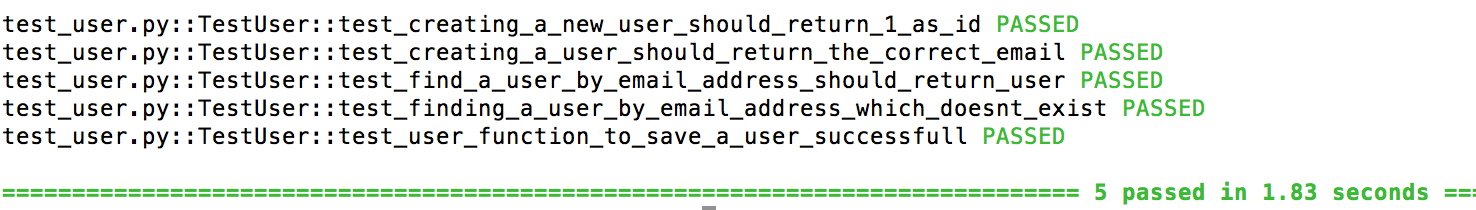
\includegraphics[width=\textwidth]{images/unit_test_user}
  \caption{Example Unit test for the user class. Each of the tests pass}
  \label{fig:unit_user}
\end{figure}

Figure \ref{fig:unit_user} shows an example of a selection of unit tests for the user class. Each of the tests considered one function in the user class to implement, whilst edge-case tests were considered too.

The testing as a whole could be considered part of the design of the application: after the story was broken down into a series of tasks, and the analysis of CRC cards was completed each function was written as a test. Whilst doing the unit tests, the core design decisions on what would be returned and what is expected of a function was decided - as well as descriptive function names. Each test would compare the output of the function with the expectation of the output.

Over the course of the project, the unit tests evolved and so did the model classes. The unit tests were the core foundations for the application to be built upon. With adopting this approach, there are times which the unit tests need to be refactored to reflect the new design. Therefore, by keeping up to date with the design it would act as a form documentation for the system.

An excerpt of unit tests can be found in Appendix \ref{appendix:test_results}, Section \ref{test:unit}.

\subsection{Integration testing}
As the application made use of routing then tests to ensure the correct response codes were being returned was important. When breaking down the story, it was identified if there needed to be new routes tested or if the controller would change its functionality. If so these were the first tests written for the routing sections, and implemented from the design considerations in Section \ref{design:urls}.

The integration tests were important as it was testing the model components and data being brought together. The tests ensured that the different systems were compatible and performed the correct operations. Routing tests consisted of checking that the response codes were correct, any redirects were correctly redirected.

An example integration test from the activity diagram shown in Section \ref{design:user_interaction}, would be: once a POST request has been made to add note URL did the note correctly get saved with the associated metadata. This test would check for the persistence of the note, and that both data can be sent to the route and it had a specific outcome.

Appendix \ref{appendix:test_results} Section \ref{appendix:integration_tests} shows a selection of integration tests.

\subsection{Handling sessions}
Session handling was a lot more complex than first anticipated. Throughout the application sessions are used to handle server-side states of the system: i.e, is the user logged in.

When testing the session it would attempt to be tested in an isolated environment, like the unit tests. Integration tests threw a lot of errors when testing with sessions. For example, if a route was accessed but the session was not set then the test would error. To overcome this, sessions needed to be modified in the tests. As the integration tests were using Flask's \texttt{test\_client} context, then modifying the sessions was a little easier. Flask had a solution to testing the session handling \cite{citeulike:14020609}.

\begin{lstlisting}[language=python, label={lst:session}, breaklines, columns=fullflexible, keywordstyle=\color{blue}, basicstyle=\normalsize\ttfamily, caption= {An example of how sessions were handled and modified in the tests.}]
  with self.client.session_transaction() as session:
          session['user_id'] = self.user_id
\end{lstlisting}

Figure \ref{lst:session}, displays an example on how the session had to be modified in the integration tests. After the session transaction context has exited then the session has been modified for that test.

Acceptance testing initially proved to be problematic. The acceptance tests would not acknowledge that the session had been modified, like in Figure \ref{lst:session}, causing the tests to error. As there was a lack of documentation it was decided that the session helper would be mocked. By mocking the responses in the \texttt{create\_app} function, it enabled the sessions to be modified, allowing the acceptance tests to be run.
\section{Acceptance testing}
Acceptance tests were created to check that the correct output was displayed for using the system. These tests ensured that the system integrated together, rendering the correct content and executing the correct operations.

Each user story was broken down and throughout the testing process the acceptance tests would be the final tests added to check that the functionality was completely integrated. Selenium for Python \cite{citeulike:14020625} was used as the acceptance tool for interacting with the web page. By interacting with the document object model (DOM) it was able to test any dynamic HTML rendered.

Before the tests were written a browser type was selected for Selenium; Chrome, Firefox, or a headless browser (via phantomJS) could be selected. The headless browser was selected as it can perform the same interactions but it does not display a graphical UI, and is a little quicker \cite{citeulike:13983611}.

Acceptance tests were created to extend the \texttt{LiveServerClass} from the Flask-Testing package. This differs from the Integration and Unit tests as those tests subclass \texttt{TestClass}. Using the \texttt{LiveServerClass} creates a server instance so Selenium can access it easily. This removes the need for an external Selenium sever.

After the unit tests were written for a feature, the acceptance tests were added to ensure the systems combined together successfully. An example of an acceptance test from the user-story, search for a note is as follows:
\begin{enumerate}
  \item Go to page /search.
  \item Find the search field.
  \item Enter the text ``CS31310''
  \item Click submit
  \item Find ``searched-item'' from the DOM.
  \item Return whether it equals ``CS31310''
\end{enumerate}

Acceptance are unlike any of the other testing techniques used in the application; rather than testing for underlying functionality the principle is to test the content to the user is displayed correctly. The tests are evaluated against the content displayed.

Another example of Selenium tests being beneficial was checking the output colour from Tesseract's confidence. The logic in the view file determined the colour and Selenium was able to confirm the logic was correct.

\begin{figure}[h!]
  \centering
  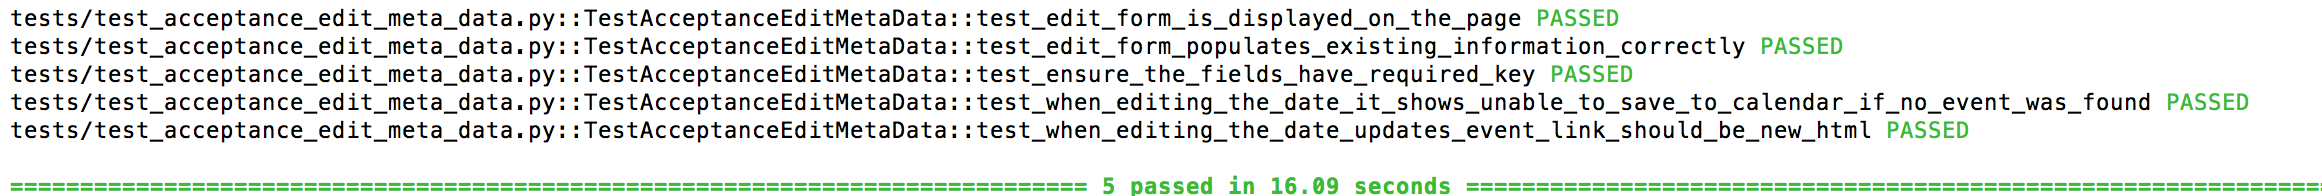
\includegraphics[width=\textwidth]{images/acceptance_test_1}
  \caption{An example of the acceptance tests running. It shows that the time to run the tests have increased considerably.}
  \label{fig:acceptance_test_1}
\end{figure}

In Figure \ref{fig:acceptance_test_1} it shows that the time to run to five tests increased to 16.09 seconds; one of the disadvantages is the time taken to run the test-suite. Due to the complexity with loading data correctly to the view file, then these tests are imperative to ensure the user expects to see the correct content. For a selection of acceptance tests refer to Appendix \ref{appendix:test_results}, Section \ref{appendix:acceptance}.

Overall, the acceptance tests were incrementally developed helping to aid the design of the frond-end through a series of tests and they proved an important tool when testing.

\section{User Testing}
As the application was aiming to solve a problem, a set of potential users were asked to perform a user study of the application. Their responses was analysed and their opinions on whether the software met their aims was collated.

Prior to the actual scheduled user-testing, feedback was given regarding the displaying of the Tesseract output confidence. These informal comments were along the lines of: ``It would be great if you could click the identified text and it would automatically populate the text boxes''. This was then implemented as a result from pre-user testing.

Further issues which were identified during the user testing were:
\begin{itemize}
  \item Uploading a JPG image off a phone, which does not have the correct date-time exif-data key causes the application to fail.
  \item Uploading an image with a previously uploaded filename caused the application to display the old file.
\end{itemize}

These issues were caught and modified and changed from areas of the design which were potentially over looked.

\begin{figure}[h!]
  \centering
  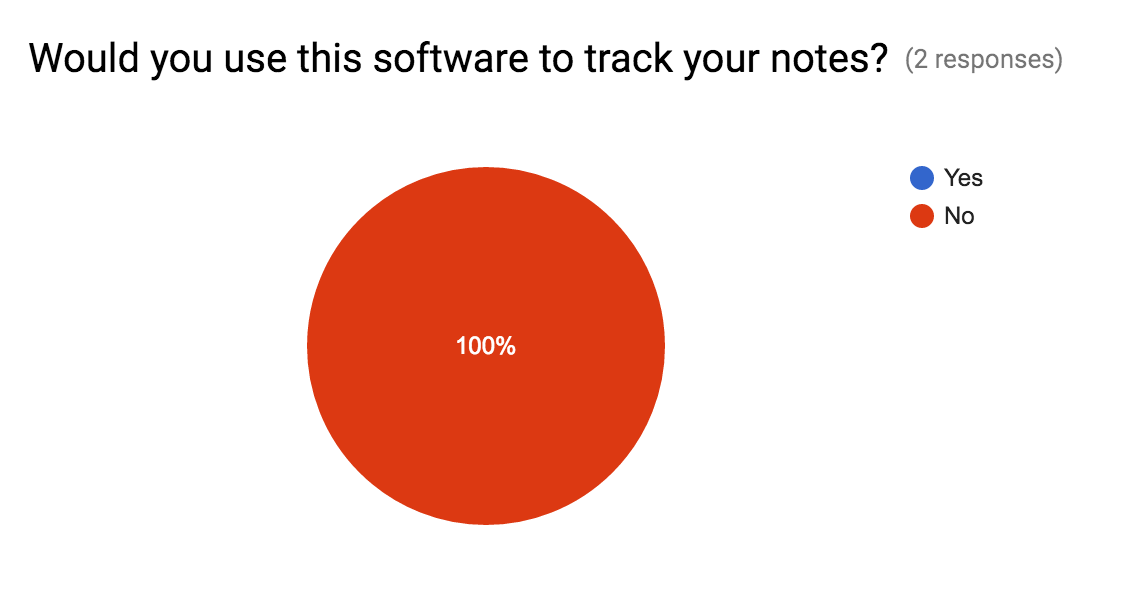
\includegraphics[scale=0.5]{images/user_response}
  \caption{A pie chart from the Google forms questionnaire \cite{citeulike:14025272} that the users conducted showing that they would not use the application for archiving their notes.}
  \label{fig:user_response}
\end{figure}

An interesting reflection from the user study was that participants would not use the application, as shown in Figure \ref{fig:user_response}. They were quick to defend the applications quality, but the use-case for them taking notes was not present. They much preferred to write up their notes from the lecture for memory retention, so the application would not benefit them.

There were positives to come out of the user testing where users agreed that it was simple to use and easy to navigate around and the websites presentation was well received. See Appendix \ref{} for user study results.

\section{Tesseract testing}
As Tesseract was a training process no additional code was written for this. An analysis of how well Tesseract learnt as it progressed through the training process can be represented.

\begin{figure}[h!]
  \centering
  \includegraphics[scale=0.6]{images/tesseract_testing}
  \caption{A simple framework showing the steps of analysing each of the training examples for a statistical measure for how successful the training process was.}
  \label{fig:tesseract_framework}
\end{figure}

Figure \ref{fig:tesseract_framework} shows a simple framework for analysing how well Tesseract trained the data. After the statistics has been collated a graph was constructed to show data collected.


Before the Tesseract training can be analysed it is worth acknowledging the test results from the spike work conducted at the start of the project which compares different thresholding algorithms on which one was suitable.

\begin{table}[H]
\centering
\begin{tabular}{ ||p{3cm}||p{3cm}|p{3cm}|p{3cm}||  }
 \hline
 \multicolumn{4}{||c||}{Image pre-processing Spike work - Correct Results vs Characters on the page} \\
 \hline
      Paper type & Greyscale & Original & Threshold\\
 \hline
  Blue-Lined &  6.75\% & 13.5\% & 28.0\% \\
  Lined & 0\% & 25\% & 13.5\% \\
  Plain & 0\% & 0\% & 23\% \\
 \hline
\end{tabular}
\caption{Table showing the results of non trained handwriting on different adaptive thresholding algorithms.}
\label{table:pre-training}
\end{table}

Table \ref{table:pre-training} shows the results from the experiments conducted to analyse which thresholding algorithm works efficiently. The result clearly show that the thresholding image yielded the best accuracy. As a result, thresholding was used. The rest of the section discusses the Tesseract training performance on adaptive threshold with Gaussian. For further statistics on this test see Appendix \ref{tesseract:spike_results}.


\begin{figure}[h!]
  \centering
\begin{tikzpicture}
\begin{axis}[
    title={Tesseract Training examples compared to their success rate of characters identified vs correct characters},
    title style={text width=\textwidth, align=center},
    xlabel={Training example},
    ylabel={Success rate (\%) },
    xmin=0, xmax=100,
    ymin=0, xmax = 100,
    ytick={0,20,40,60,80,100},
    xtick={0, 9,18,27,36,45,54,63, 72, 81 , 90 , 99},
    xticklabels={1, 2, 3, 4, 5, 6, 7, 8, 9 , 10 , 11 ,12 },
    legend pos=north west,
    ymajorgrids=true,
    grid style=dashed,
]

\addplot[
    color=black,
    mark=square,
    ]
    coordinates {
    (0, 61.4035087719298)(9, 72.2222222222222)(18, 81.1594202898551) (27, 79.1044776119403)(36, 69.7916666666667)(45, 74.6376811594203) (54, 78.5276073619632)(63, 69.75)(72, 78.7878787878788)(81, 66.3341645885287)(90, 65.5737704918033)(99, 75.414364640884)
    };

\addplot [thick, red] table[y={create col/linear regression}]{
    0 61.4035087719298
    9 72.2222222222222
    18 81.1594202898551
    27 79.1044776119403
    36 69.7916666666667
    45 74.6376811594203
    54 78.5276073619632
    63 69.75
    72 78.7878787878788
    81 66.3341645885287
    90 65.5737704918033
    99 75.414364640884
    };
\end{axis}
\end{tikzpicture}
\caption{A line-graph showing the success rate of the Tesseract training results over 12 examples. The trend line shows an almost horizontal linear line.}
\label{fig:tesseract_graph}
\end{figure}

Figure \ref{fig:tesseract_graph} shows the output analysed from the Tesseract training using the segmentation algorithm discussed in Section \ref{imp:image_proces}. It shows each training example with an associated success rate for the characters identified. The conclusions clearly show that there is no improvement from the Tesseract output after around the 3rd example. A horizontal linear regression line shows that it has peaked at around 72\% correct recognition rate. Refer to appendix \ref{appendix:tesseract}, section \ref{appendix:tesseract_table} for the full statistics.

\vspace{2em}
\section{Image threshold testing}
A methodical testing approach would not appropriate for the segmentation script development, as it was predominantly spike work.

The testing was conducted at more of a visual level, checking the output of the image to see if the image has been binarised successfully. Once the script had been developed to a suitable level then the spike work would stop and testing would begin.

The code was re-written following a TDD approach, although a lot of the code was interacting with OpenCV it was assumed that these functions had been reliably tested. Nevertheless, testing for the script was produced and checks such as checking for black pixels in the image was written.

For examples of the test images used for the image threshold used as training examples for the Tesseract engine, see Appendix \ref{tesseract:training}.
